\subsection{UC5 - Visualizzazione errore}
\label{sub:uc5}

% TODO: Modifica immagine
\begin{figure}[h]
    \centering
    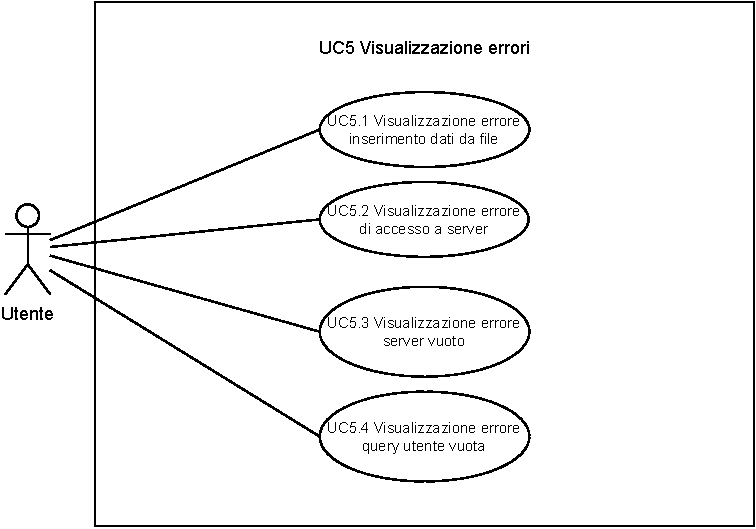
\includegraphics[width=0.7\textwidth]{componenti/casi-duso/diagrammi/UC5.pdf}
    \caption{Diagramma rappresentante UC5}
    \label{fig:UC5}
\end{figure}

\begin{itemize}
    \item \textbf{Descrizione}: L'utente visualizza un messaggio di errore relativo ad un'operazione non eseguita 
    correttamente;

    \item \textbf{Attore primario}: Utente;
    
    \item \textbf{Precondizione}:   Un'operazione non è stata eseguita correttamente; 

    \item \textbf{Postcondizione}:  Viene visualizzato un messaggio di errore relativo all'operazione;
    
    \item \textbf{Scenario Principale}:
    \begin{enumerate}
        \item Viene visualizzato il messaggio di errore;
        \item L'utente conferma la presa visione dell'errore che si è verificato.
    \end{enumerate}

    \item \textbf{Generalizzazioni}:
    \begin{enumerate}
        \item Visualizzazione errore inserimento dati da file (\hyperref[sub:uc6]{UC6});
        \item Visualizzazione errore di accesso a server (\hyperref[sub:uc7]{UC7});
        \item Visualizzazione errore server vuoto (\hyperref[sub:uc8]{UC8})
        \item Visualizzazione errore query utente vuota (\hyperref[sub:uc9]{UC9});
        \item Visualizzazione errore modifica metadato di visibilità (\hyperref[sub:uc10]{UC10}).
    \end{enumerate}

\end{itemize}

%TODO: Cambiare numerazione? Al momento ha senso da una parte ma non è giustificata qui visto che sottocasi non sono veri e propri.

\subsubsection{UC6 - Visualizzazione errore inserimento dati da file}
\label{sub:uc6}
\begin{itemize}
    \item \textbf{Descrizione}: L'utente visualizza un messaggio di errore dopo aver caricato un file CSV non corretto 
    o vuoto;

    \item \textbf{Attore primario}: Utente;
    
    \item \textbf{Precondizione}:   L'utente carica un file CSV non corretto o vuoto (\hyperref[ssub:uc1.2]{UC1.2});

    \item \textbf{Postcondizione}:  Viene visualizzato un messaggio di errore relativo alla non correttezza del file 
    caricato;

    \item \textbf{Scenario principale}:
    \begin{enumerate}
        \item Viene visualizzato un messaggio d'errore relativo alla non correttezza del file caricato;
        \item L'utente conferma la presa visione dell'errore.
    \end{enumerate}

\end{itemize}


\subsubsection{UC7 - Visualizzazione errore di accesso a server}
\label{sub:uc7}
\begin{itemize}
    \item \textbf{Descrizione}: L'utente visualizza un messaggio di errore dopo il fallimento dell'accesso
    al server indicato;

    \item \textbf{Attore primario}: Utente;
    
    \item \textbf{Precondizione}:   La connessione con il server indicato dall'utente fallisce 
    (\hyperref[par:uc1.3.1]{UC1.3.1});

    \item \textbf{Postcondizione}:  Viene visualizzato un messaggio di errore relativo al fallimento della connessione 
    con il server indicato dall'utente;

    \item \textbf{Scenario principale}:
    \begin{enumerate}
        \item Viene visualizzato un messaggio d'errore relativo alla mancata connessione al server indicato dall'utente;
        \item L'utente conferma la presa visione dell'errore.
    \end{enumerate}
\end{itemize}



\subsubsection{UC8 - Visualizzazione errore server vuoto}
\label{sub:uc8}
\begin{itemize}
    \item \textbf{Descrizione}: L'utente visualizza un messaggio di errore per la mancanza di database o di dataset 
    validi nel server connesso;

    \item \textbf{Attore primario}: Utente;
    
    \item \textbf{Precondizione}:   Il server connesso non presenta database oppure quelli presenti sono vuoti 
    (\hyperref[par:uc1.3.2]{UC1.3.2});

    \item \textbf{Postcondizione}:   Viene visualizzato un messaggio di errore relativo alla mancanza di database o di 
    dataset validi nel server connesso;

    \item \textbf{Scenario principale}:
    \begin{enumerate}
        \item Viene visualizzato un messaggio d'errore relativo alla mancanza di database o di dataset validi nel 
        server connesso;
        \item L'utente conferma la presa visione dell'errore.
    \end{enumerate}

\end{itemize}


\subsubsection{UC9 - Visualizzazione errore query utente vuota}
\label{sub:uc9}
\begin{itemize}
    \item \textbf{Descrizione}: L'utente visualizza un messaggio di errore per l'esecuzione di una query sul database 
    esterno che ha restituito un dataset non valido;

    \item \textbf{Attore primario}: Utente;
    
    \item \textbf{Precondizione}:   La query eseguita ha restituito un dataset non valido 
    (\hyperref[par:uc1.3.2]{UC1.3.2});

    \item \textbf{Postcondizione}:   Viene visualizzato un messaggio di errore relativo alla restituizione di un dataset non valido dall'esecuzione di una query sul database esterno;
    
    \item \textbf{Scenario principale}:
    \begin{enumerate}
        \item Viene visualizzato un messaggio d'errore relativo relativo alla restituizione di un dataset non valido 
        dall'esecuzione di una query sul database esterno;
        \item L'utente conferma la presa visione dell'errore.
    \end{enumerate}

\end{itemize}

\subsubsection{UC10 - Visualizzazione errore modifica metadato di visibilità}
\label{sub:uc10}

\begin{itemize}
    \item \textbf{Descrizione}: L'utente visualizza un messaggio di errore per la modifica impropria di un metadato di 
    visibilità;

    \item \textbf{Attore primario}: Utente;
    
    \item \textbf{Precondizione}:   Viene impostato un metadato di visibilità a "nascosta", con meno di due dimensioni 
    visibili;

    \item \textbf{Postcondizione}:   Viene visualizzato un messaggio di errore relativo alla modifica impropria di un 
    metadato di visibilità;

    \item \textbf{Scenario principale}:
    \begin{enumerate}
        \item Viene visualizzato un messaggio di errore relativo alla modifica impropria di un metadato di visibilità;
        \item L'utente conferma la presa visione dell'errore.
    \end{enumerate}
\end{itemize}